\documentclass{article} % For LaTeX2e
\usepackage{nips13submit_e,times}
\usepackage{hyperref}
\usepackage{url}
\usepackage{graphicx}
\graphicspath{ {images/} }
%\documentstyle[nips13submit_09,times,art10]{article} % For LaTeX 2.09


\title{An Investigation of Classification Techniques For Handwritten Digit Recognition}


\author{
Deric Pang \\
\texttt{dericp@cs.washington.edu} \\
\And
Saidutt Nimmagadda \\
\texttt{nimmas@cs.washington.edu} \\
}

% The \author macro works with any number of authors. There are two commands
% used to separate the names and addresses of multiple authors: \And and \AND.
%
% Using \And between authors leaves it to \LaTeX{} to determine where to break
% the lines. Using \AND forces a linebreak at that point. So, if \LaTeX{}
% puts 3 of 4 authors names on the first line, and the last on the second
% line, try using \AND instead of \And before the third author name.

\newcommand{\fix}{\marginpar{FIX}}
\newcommand{\new}{\marginpar{NEW}}

\nipsfinalcopy % Uncomment for camera-ready version

\begin{document}

\maketitle

\begin{abstract}
  TODO
\end{abstract}

\section{Introduction}
TODO

\section{Project Description}
\subsection{Goal}

Our goal for this project is quite simple---we want to
take pixel data from images of hand-drawn digits
and classify them as a number from 0 to 9.

\subsection{Data}

The data for our project was taken from the MNIST dataset. As written on a
Kaggle competition using the MNIST dataset, ``The MNIST
('Modified National Institute of Standards and Technology') dataset
is a classic within the Machine Learning community that has been extensively
studied. More detail about the dataset, including Machine Learning algorithms
that have been tried on it and their levels of success, can be found at
\href{http://yann.lecun.com/exdb/mnist/index.html}{http://yann.lecun.com/exdb/mnist/index.html}.''

Each handwritten digit is vectorized. Each vector is composed of a label which
represents the label classification (i.e. numbers from 0 to 9) and 783 pixel
features of integer values between 0 and 255. Since all
of the data is already normalized and centered, we did not need to take those
steps ourselves to start building models against. The training data set
consists of 60,000 data points, while the test set consists of 10,000 data
points.

The specific flavor of the MNIST dataset that we used came from
\href{https://pjreddie.com/projects/mnist-in-csv/}{https://pjreddie.com/projects/mnist-in-csv/}
where the data is formated as a CSV.

\section{First Considerations}
\subsection{Machine Learning Techniques}
TODO

\subsection{Related Work}
Before we began implementing any classifiers, we wanted to investigate what
material already existed in the domain of digit recognition. We discovered
that digit recognition, especially on the MNIST database, is an extremely well
studied problem. As such, we had no trouble finding a plethora of detailed
papers.

Going into the project, we had intuition that the most accurate classifier we
could build was a convolutional neural network. This was confirmed in most of
the related work [1 - 3].
However, we wanted to determine which techniques would be the most insightful,
interesting, and performant to implement for our project even though the
readings pointed out a clear state-of-the-art.

We found from the
conclusions of Lecun [1] that the k-Nearest Neighbors classifier would not
only pose serious scaleability difficulties when it came to runtime and memory
usage, but it would also be a comparatively unreliable classifier. We decided
that it would be interesting to see just how difficult it would be to deal with
the runtime and what kind of accuracy we could achieve with limited
computation resources.

We also saw that according to Maji [2], ``with improved features a low
complexity classifier, in particular
an additive-kernel SVM, can achieve state of the art performance.'' This
inspired us to implement a support vector machine as a lightweight, high
accuracy classifier.

%Our findings from the milestone portion of the project confirms this, with our implementation
%of k-NN taking a good amount of time (roughly 5 minutes) to run over less than
%10 percent of the total dataset. In addition, we only achieved classification
%errors of roughly 10 
%to 20 percent. When we implement a convolutional neural network, like LeCun did
%in his paper, we expect a decrease in runtime and memory usage (which
%would promote scaleability), as well as a large decrease in classification error.

\section{Approach}

\subsection{Baselines}
We used scikit-learn [6] to implement baselines for the $k$-NN classifier and the SVM.
Even though scikit-learn is presumably optimized very well, these classifiers took a very
long time to train and evaluate. As a result, we tuned hyperparameters with only
17\% of our training data. Once we settled upon optimal hyper
parameters, we trained the scikit-learn $k$-NN and SVM on 25\% of the training set and evaluated
them on the entirety of the test set.

%After implementing the baselines, we implemented the algorithms themselves.
%For each high level algorithm, we implemented different refinements and ran
%cross-validation in order to get a diverse array of data for a diverse array of
%techniques. We kept a high scope by having multiple algorithms, and we kept a
%high depth by tinkering with each algorithm. Finally, we used TensorFlow to
%implement a convolutional neural network. We knew from the readings we’d read
%that a CNN would perform optimally, and we wanted to have our own optimal
%baseline to compare our results to.

\subsection{Evaluation}
To tune hyperparameters, we used cross-validation with random 80-20 splits. We
consistently report the validation errors from the cross-validation and the test
error on the MNIST test set.

\subsection{$k$-Nearest Neighbors}
We implemented a $k$-nearest neighbors ($k$-NN) classifier using
$k$-nearest neighbors regression. 
The first issue we ran into was the intractable runtime needed to run $k$-NN
over the large training set of 60,000 images. Given runtime constraints,
we ran the algorithm on 10\% of the training set.
For each value of $k$, we found the classification error on the validation set.

TODO these graphs say classification error when it should be VALIDATION error.

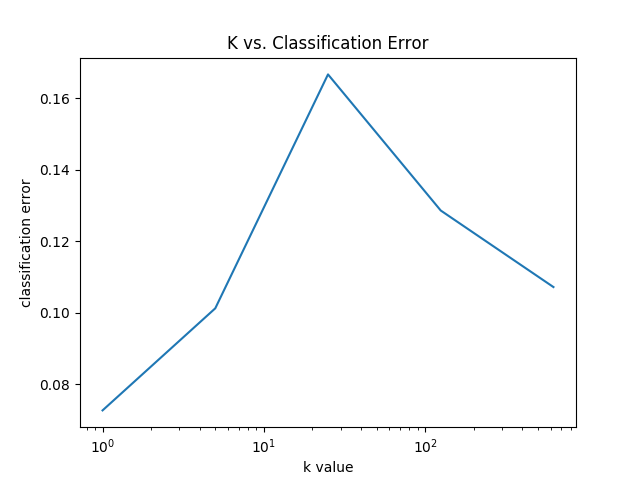
\includegraphics[width=\textwidth]{k-nn.png}

Surprisingly, we can see that with $k = 1$ we achieve the lowest classification
error. This is most likely due to the lack of a kernel to weigh the points
according to how far they are from the query. We would expect that as $k$
increases, our classification error would decrase. However, without a
proper kernel to weigh the data points, this is unlikely.

We first tackled nearest neighbor regression. For baselining, we used
the scikit-learn NearestNeighbors functionality. Rather than choosing a
particular nearest neighbors algorithm, we let scikit-learn decide which
nearest neighbors algorithm to use after analysis of the training model.
Algorithms available include brute force, the K-D tree, and Ball tree.
The latter two trade precision off for efficiency by using heuristics to
prune which points are considered when evaluating “nearest neighbors.” The
decision on which algorithm to use is based on the number of samples, the
structure of the data (e.g. sparsity, intrinsic dimensionality), the number
of neighbors requested for a query point, and the number of query points.
The baseline library ended up choosing the K-D tree algorithm because of
the k values we cross validated over, and the one we ended up using for
our final model, being less than N/2. 
We ran cross-validation over a small subset of our training set (1/10th
of the training set). Running cross validation over a set of k values from
1 to 625, we found that a k of 1 minimized our validation error. 

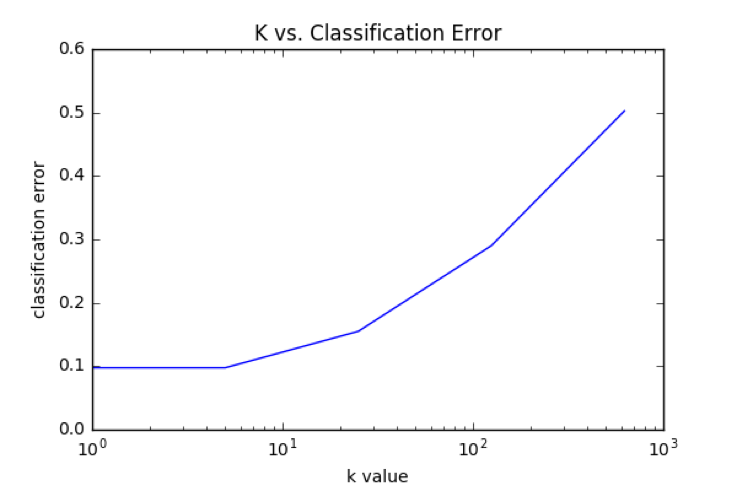
\includegraphics[width=\textwidth]{sklearn-knn-cv.png}

After running cross validation on our baseline, we implemented our own
K-Nearest Neighbors algorithm. We used a brute force algorithm that scans
every point in the training set to find the k neighbors with the lowest
Euclidean distances from the query point. Then, amongst those k neighbors,
we found the classification with the lowest average Euclidean distance from
the query point. That classification was the classification we’d assigned to
the query point.

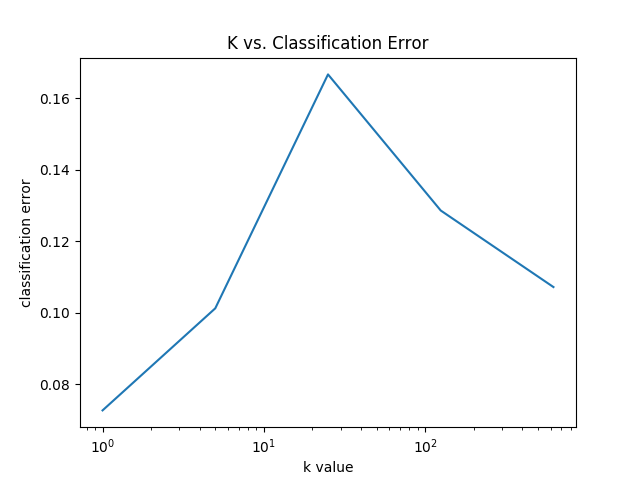
\includegraphics[width=\textwidth]{k-nn.png}

We ran cross-validation over a small subset of our training data (once again,
1/10th).
The results backed up the results from the library implementation with a k
of 1 minimizing our validation error. 
Afterwards, we implemented a Gaussian kernel and classified query points
based off of the Nadaraya Watson Kernel Weighted Average. Instead of finding
the k nearest neighbors to classify a query point, we used this Kernelized
Regression to calculate the classification for each query point.

TODO include kernel formulation here

Since we didn’t have to just find the k nearest neighbors, but instead
iterated through every point and kernelized its distance as a weight to
its classification, we had to tune our bandwidth value $\lambda$ rather than a k.
As a result of overflow and underflow errors, we could only test a range
of bandwidths from $10^4$ to $10^6$. 

TODO this x-axis is mislablbed, it should be BANDWIDTH

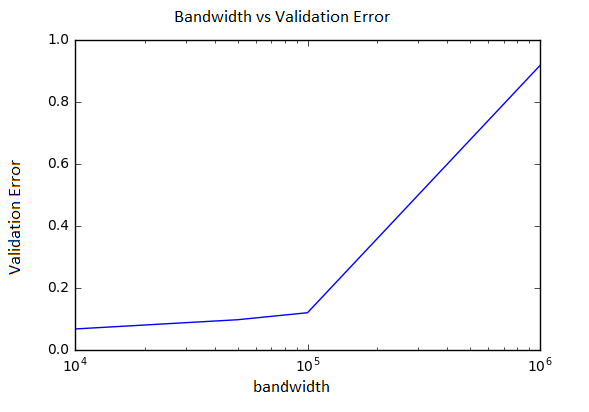
\includegraphics[width=\textwidth]{knn-kernel-bandwidth-cv.png}

Running cross validation on 1/10th of our training set, we found that a
bandwidth of 104 not only avoided overflow errors, it also minimized validation error.

\subsection{SVM}
We then tackled Support Vector Machines. For baselining,
we used scikit-learns LinearSVC and SVC functionality. The
former trains a Support Vector Machine until convergence with
a Linear kernel, and the latter with a Radial Basis function kernel. 

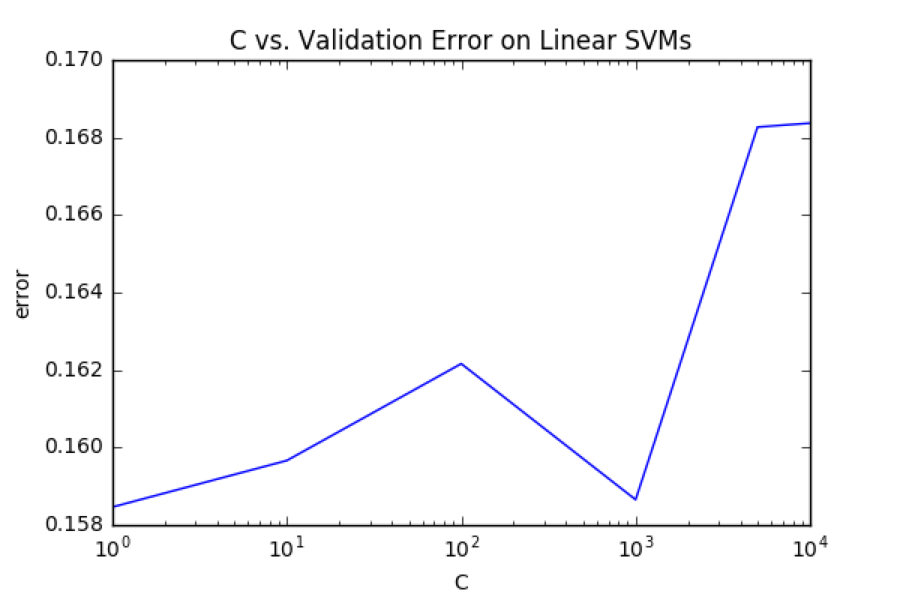
\includegraphics[width=\textwidth]{sklearn-svm-c-cv.png}

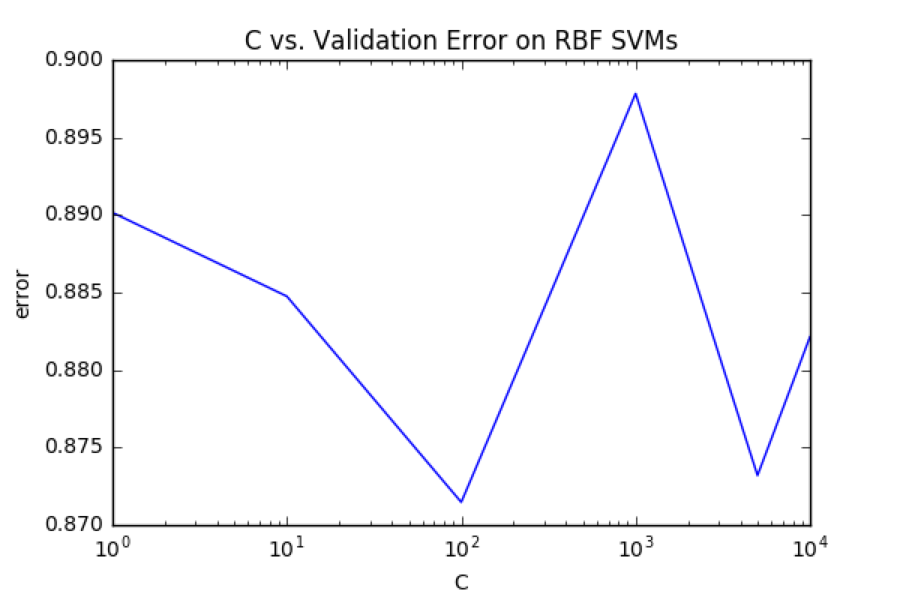
\includegraphics[width=\textwidth]{sklearn-svm-kernel-c-cv.png}

Running cross-validation for each C value over a small subset of
the training set (10000 rows), we found that C values of 1 and 100
minimized validation error in the Linear and RBF SVMs respectively.
This was surprising to us, especially the former C-value, and we
suspected after some tinkering around that the differences in
validation error can be ascribed to differences in the validation
blocks’ data rather than differences in C value. Nonetheless, we
used those respective C-values for creating our model against the
the training data and running it against the test data. 


\subsection{CNN}
TODO

\section{Results}

\subsubsection*{References}

\small{
  [1] LeCun, Yann, et al. "Comparison of learning algorithms for handwritten
  digit recognition." International conference on artificial neural networks.
  Vol. 60. 1995.	

  [2] Maji, Subhransu, and Jitendra Malik. "Fast and accurate digit
  classification." EECS Department, University of California,
  Berkeley, Tech. Rep. UCB/EECS-2009-159 (2009).

  [3] Sundaresan, Vishnu, and Jasper Lin. "Recognizing Handwritten Digits and
  Characters." (1998).

  [4] Shalev-Shwartz, Shai, Yoram Singer, and Nathan Srebro. "Pegasos: Primal
  estimated sub-gradient solver for svm." Proceedings of the 24th international
  conference on Machine learning. ACM, 2007.

  [5] Rahimi, Ali, and Benjamin Recht. "Random Features for Large-Scale Kernel
  Machines." NIPS. Vol. 3. No. 4. 2007.

  [6] Pedregosa, Fabian, et al. "Scikit-learn: Machine learning in Python."
  Journal of Machine Learning Research 12.Oct (2011): 2825-2830.
}

\end{document}
